\section{eo\-Es\-Simple$<$ Fit $>$ Class Template Reference}
\label{classeo_es_simple}\index{eoEsSimple@{eoEsSimple}}
Simple Evolution Strategy.  


{\tt \#include $<$eo\-Es\-Simple.h$>$}

Inheritance diagram for eo\-Es\-Simple$<$ Fit $>$::\begin{figure}[H]
\begin{center}
\leavevmode
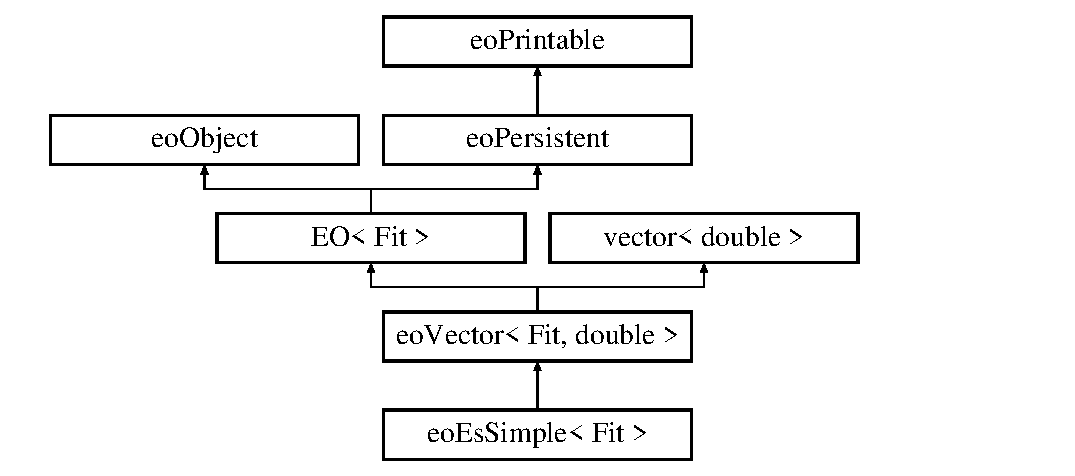
\includegraphics[height=5cm]{classeo_es_simple}
\end{center}
\end{figure}
\subsection*{Public Types}
\begin{CompactItemize}
\item 
typedef double {\bf Type}\label{classeo_es_simple_w0}

\end{CompactItemize}
\subsection*{Public Member Functions}
\begin{CompactItemize}
\item 
virtual std::string {\bf class\-Name} () const 
\begin{CompactList}\small\item\em Return the class id. \item\end{CompactList}\item 
void {\bf print\-On} (std::ostream \&os) const \label{classeo_es_simple_a2}

\begin{CompactList}\small\item\em printing... \item\end{CompactList}\item 
void {\bf read\-From} (std::istream \&is)\label{classeo_es_simple_a3}

\begin{CompactList}\small\item\em reading... \item\end{CompactList}\end{CompactItemize}
\subsection*{Public Attributes}
\begin{CompactItemize}
\item 
double {\bf stdev}\label{classeo_es_simple_o0}

\end{CompactItemize}


\subsection{Detailed Description}
\subsubsection*{template$<$class Fit$>$ class eo\-Es\-Simple$<$ Fit $>$}

Simple Evolution Strategy. 

One of the more simple evolution strategies, sporting just a single stdeviation for the entire chromosome. For more advanced versions see also {\bf eo\-Es\-Stdev}{\rm (p.\,\pageref{classeo_es_stdev})} {\bf eo\-Es\-Full}{\rm (p.\,\pageref{classeo_es_full})}

\begin{Desc}
\item[See also:]{\bf eo\-Es\-Stdev}{\rm (p.\,\pageref{classeo_es_stdev})} {\bf eo\-Es\-Full}{\rm (p.\,\pageref{classeo_es_full})} \end{Desc}




Definition at line 42 of file eo\-Es\-Simple.h.

\subsection{Member Function Documentation}
\index{eoEsSimple@{eo\-Es\-Simple}!className@{className}}
\index{className@{className}!eoEsSimple@{eo\-Es\-Simple}}
\subsubsection{\setlength{\rightskip}{0pt plus 5cm}template$<$class Fit$>$ virtual std::string {\bf eo\-Es\-Simple}$<$ Fit $>$::class\-Name (void) const\hspace{0.3cm}{\tt  [inline, virtual]}}\label{classeo_es_simple_a1}


Return the class id. 

\begin{Desc}
\item[Returns:]the class name as a std::string \end{Desc}


Reimplemented from {\bf EO$<$ Fit $>$} {\rm (p.\,\pageref{class_e_o_z10_0})}.

Definition at line 50 of file eo\-Es\-Simple.h.

The documentation for this class was generated from the following file:\begin{CompactItemize}
\item 
eo\-Es\-Simple.h\end{CompactItemize}
